\section{Experimental Evaluation}
\label{sec:experiments}

The experiments examine three questions: whether the proposed hierarchy
reduces computation energy while meeting the service requirements;
whether its policy remains effective when the deadline distribution
changes; and which components account for the observed behavior.
Energy, deadline service attainment, and reliability attainment are
reported separately to distinguish valid energy savings from reductions
obtained by violating constraints.

\subsection{Experimental Setup}
\label{subsec:experiment_setup}

\subsubsection{Workflows and Resource Configurations}

The simulator uses DAG topologies from five scientific workflow families:
CyberShake, Epigenomics, Inspiral, Montage, and SIPHT. The Small pool
contains five templates with 24--30 tasks. The Medium pool contains these
five templates and five larger templates, giving 24--58 tasks per
workflow. Thus, Medium is a cumulative template pool rather than a
collection consisting exclusively of larger DAGs. A template is sampled
uniformly for each workflow. Task workloads and edge data volumes are
sampled uniformly from $[0.5,20]\times10^9$ cycles and $[1,30]$ MB,
respectively. The topologies are benchmark-derived, whereas these
execution and communication parameters are synthetic.

Each workload realization contains 20 dynamically arriving workflows.
Interarrival times are exponentially distributed with rate
$0.1\ \mathrm{s}^{-1}$, corresponding to a mean interval of 10 s.
Table~\ref{tab:experiment_scenarios} defines a two-by-two design involving
workload size and relative resource provision. Expanding S26 to S37
increases the server count from 26 to 37; expanding M37 to M53 increases
it from 37 to 53. These changes apply similar expansion factors to both
workload scales while approximately preserving the edge--cloud ratio.
All policies are trained for their own workload--resource configuration;
a checkpoint with a different number of server outputs is not used as
the trained model of another configuration.

\begin{table}[t]
\centering
\caption{Workload--resource configurations. Mean task counts are averages
over the template pools, not measurements of system utilization.}
\label{tab:experiment_scenarios}
\footnotesize
\setlength{\tabcolsep}{4pt}
\renewcommand{\arraystretch}{1.08}
\begin{tabular}{@{}llrrrr@{}}
\toprule
ID & Pool & Tasks & Mean & Edge & Cloud \\
\midrule
S26 & Small & 24--30 & 27.6 & 20 & 6 \\
S37 & Small & 24--30 & 27.6 & 28 & 9 \\
M37 & Medium & 24--58 & 39.3 & 28 & 9 \\
M53 & Medium & 24--58 & 39.3 & 40 & 13 \\
\bottomrule
\end{tabular}
\end{table}

The common resource model contains three edge profiles and two cloud
profiles, listed in Table~\ref{tab:experiment_resources}. Edge profiles
are allocated approximately equally; the two cloud profiles are also
allocated approximately equally. Frequencies and the two power
components are independently perturbed by up to $\pm5\%$ around their
nominal values. Resource generation uses seed 42, so every method in a
configuration observes the same server pool. Edge--edge, edge--cloud,
and cloud--cloud links have bandwidths of 1, 0.1, and 10 Gbit/s,
respectively. The shared simulator orders dispatchable tasks by
increasing workload. Each server executes one task at a time without
preemption, as specified in Section~\ref{sec:model}.

\begin{table}[t]
\centering
\caption{Nominal server profiles. Power components follow
\eqref{eq:task_energy}; fault rates are measured at maximum frequency.}
\label{tab:experiment_resources}
\footnotesize
\setlength{\tabcolsep}{3pt}
\renewcommand{\arraystretch}{1.08}
\begin{tabular}{@{}lrrrr@{}}
\toprule
Profile & $F_m$ & $P_m^{\mathrm{ind}}$ & $P_m^{\mathrm{dyn}}$ & $\lambda_m^{\max}$ \\
& (GHz) & (W) & (W) & ($\mathrm{s}^{-1}$) \\
\midrule
Edge low-end & 1.80 & 3.00 & 12.80 & $10^{-5}$ \\
Edge efficient & 2.40 & 5.87 & 36.03 & $10^{-5}$ \\
Edge legacy & 2.90 & 18.06 & 102.34 & $10^{-5}$ \\
Cloud standard & 3.25 & 29.16 & 213.84 & $6\times10^{-6}$ \\
Cloud fast & 3.60 & 41.32 & 371.88 & $6\times10^{-6}$ \\
\bottomrule
\end{tabular}
\end{table}

The physical minimum frequency ratio is 0.1 and the fault-rate
sensitivity is $\kappa_m=3$. Every workflow has reliability requirement
$R_w=0.90$. The measured energy is active computation energy in joules,
not total infrastructure electricity: idle and communication energy are
excluded consistently for every method.

\subsubsection{Deadline Distributions and Metrics}

For each workflow, its relative deadline is two or three times the
full-frequency, contention-free HEFT reference makespan on the same
server pool~\cite{topcuoglu2002}. In Tight, Medium, and Loose settings,
the probabilities of choosing the two-times multiplier are 0.8, 0.5,
and 0.2, respectively; the complementary probabilities choose the
three-times multiplier. Tight therefore increases the prevalence of
less permissive deadlines rather than applying a smaller constant to
every workflow.

All models are trained under the Medium distribution. For each method
and configuration, the same selected checkpoint is evaluated under all
three distributions without further learning or multiplier adaptation.
The main results use the original, unfiltered test seeds
242000--242019. Every method uses the same 20 seeds within a condition;
no failed seed is removed or replaced. These are test workload seeds,
not independent repetitions of policy training.

We use $\Gamma=0.90$ in \eqref{eq:esp}. A realization passes the deadline
criterion if at least 18 of its 20 workflows finish on time. ESP@90 is
the fraction of the 20 test realizations passing this criterion; it is
not the average within-realization success rate. The empirical
service-level gate is ESP@90 $\geq90\%$, together with reliability
attainment of 100\%. Reliability attainment measures the proportion of
test realizations in which every workflow satisfies
$\mathcal R_w\geq R_w$. It does not mean that workflow reliability
equals one or that no physical faults could occur. Total energy is
summarized by its mean and sample standard deviation over the 20
realizations. An observed ESP of 100\% means 20 out of 20 successful
test realizations, not a guarantee of success on all future workloads.

\subsubsection{Compared Methods and Training Protocol}

Three learning-based baselines are adapted to the same simulator.
\emph{DQN-Edge}~\cite{wen2026} retains its separate time and energy
Q-estimators and attention-based combination, and performs placement
at full frequency. \emph{DReaM-DQN}~\cite{esnaashari2025dream} retains
DQN-based discrete operating-point selection, with seven frequency
levels. \emph{OOAC}~\cite{wang2025ordinal} retains its actor--critic
candidate-generation and ordinal-screening mechanism, using 100
candidates, a Top-$s$ set of 30, and five frequency levels. These are
platform-adapted implementations, not claims of unchanged reproduction
of the original experimental settings. State and reward inputs are
adapted to the common workflow, energy, deadline, and reliability
models; the characteristic learning and action-selection mechanisms
are retained. The discrete frequency indices are mapped to the
selected server's energy-efficient-to-full-frequency interval.

The proposed upper estimators use two hidden layers of 256 units;
the SAC networks use two hidden layers of 128 units. Their learning
rates are $10^{-4}$ and $3\times10^{-4}$, minibatch sizes are 256 and
128, and replay capacities are 50,000. Both levels use discount 0.99
and target-update coefficient 0.005; SAC uses entropy coefficient 0.2.
The queue calibration share is 0.20. The proposed model has a configured
ceiling of 1,200 training episodes, and the completed structural
ablations use the same ceiling. Baseline settings are recorded in
their configuration snapshots rather than assumed to have an equal
number of gradient updates. For example, the archived S26/M37
baselines have a ceiling of 1,500 episodes. Some scenario runs were
interrupted before their configured ceiling; the results use available
saved checkpoints, not an assertion that every run fully converged.

Model selection is separate from final testing. The proposed method
uses the validation blocks beginning at 542000 and 642000, with
ESP@90 $=100\%$ and full reliability attainment as a stricter selection
target, followed by energy minimization. Most baseline records use
the same two block origins but an ESP@90 target of 90\%, with either
5 or 20 realizations per block. The archived S26 DReaM run is an
exception: its legacy selection used a single 20-realization block
and mean deadline satisfaction of at least 92\%. S37 DReaM saved
checkpoints were instead re-ranked on the two 20-realization blocks;
none met the strict gate, so the largest minimum-block ESP, followed
by the lowest mean energy, determined the fallback checkpoint.
These historical differences are disclosed rather than described
as a perfectly uniform model-selection budget. No final test block
is used for checkpoint ranking.

\subsection{Energy and Service-Level Performance}
\label{subsec:main_results}

Figure~\ref{fig:main_comparison} presents energy distributions and
deadline ESP for all 12 workload--resource--deadline conditions.
Table~\ref{tab:main_energy} gives the corresponding energy means and
standard deviations. All four methods attain the reliability
requirement on every main-test realization. Reliability consequently
does not distinguish their performance under this resource setting;
the differences in empirical feasibility are driven by deadlines.

\begin{figure*}[t]
\centering
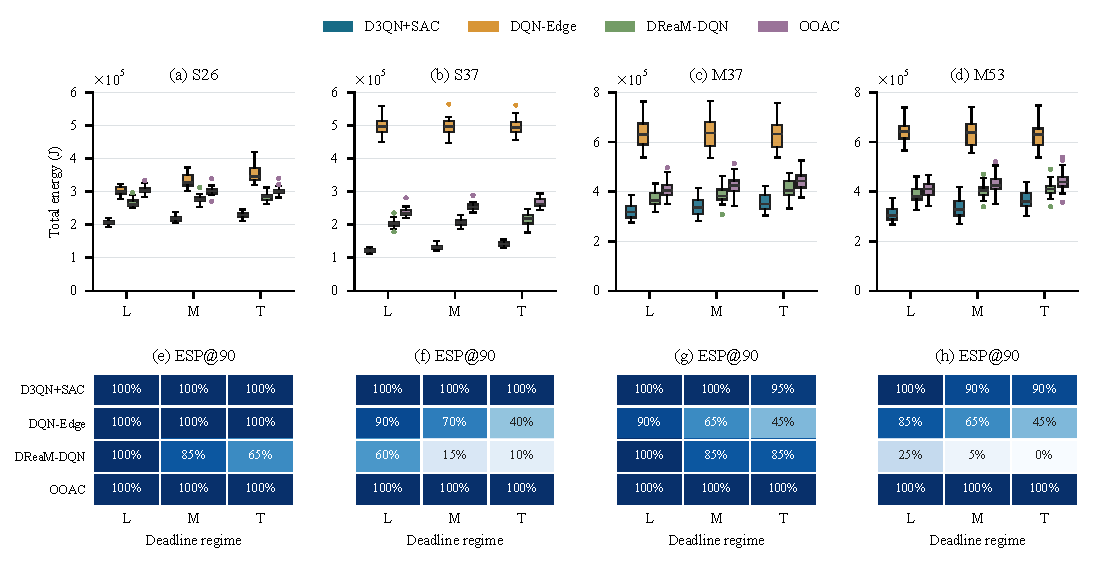
\includegraphics[width=\textwidth]{experiment_assets/main_comparison.pdf}
\caption{Main comparison on 20 matched, unseen workload seeds per
condition. Columns correspond to S26, S37, M37, and M53. In the upper
panels, boxes show the median and interquartile range of total active
computation energy; whiskers extend to the furthest observations within
1.5 interquartile ranges, and dots show observations outside the
whiskers. Lower panels report ESP@90. L, M, and T denote Loose, Medium,
and Tight deadline distributions. Reliability attainment is 100\% for
all methods. An empirical service-level feasible result requires
ESP@90 $\geq90\%$; low energy below this gate is not a feasible improvement.}
\label{fig:main_comparison}
\end{figure*}

\begin{table*}[t]
\centering
\caption{Total active computation energy (J): mean $\pm$ sample
standard deviation on the same 20 test seeds. Deadline feasibility is
reported in Fig.~\ref{fig:main_comparison}. Bold identifies the lowest
energy among empirically feasible methods in each condition.}
\label{tab:main_energy}
\footnotesize
\setlength{\tabcolsep}{7pt}
\renewcommand{\arraystretch}{1.08}
\begin{tabular}{@{}llrrr@{}}
\toprule
Scenario & Method & Loose & Medium & Tight \\
\midrule
S26 & D3QN+SAC & \textbf{206,301.27 $\pm$ 7,674.55} & \textbf{218,582.71 $\pm$ 9,004.38} & \textbf{229,668.81 $\pm$ 9,708.86} \\
 & DQN-Edge & 302,503.19 $\pm$ 12,679.50 & 333,163.60 $\pm$ 19,018.30 & 352,640.89 $\pm$ 24,430.03 \\
 & DReaM-DQN & 265,523.59 $\pm$ 12,543.93 & 277,161.73 $\pm$ 13,472.38 & 285,565.23 $\pm$ 12,765.79 \\
 & OOAC & 304,560.24 $\pm$ 12,500.09 & 302,308.85 $\pm$ 13,707.71 & 302,492.80 $\pm$ 12,803.92 \\
\midrule
S37 & D3QN+SAC & \textbf{121,572.94 $\pm$ 6,016.08} & \textbf{132,068.80 $\pm$ 7,423.62} & \textbf{142,052.08 $\pm$ 7,768.61} \\
 & DQN-Edge & 494,940.35 $\pm$ 26,979.60 & 496,496.87 $\pm$ 28,006.09 & 496,022.55 $\pm$ 29,002.06 \\
 & DReaM-DQN & 203,787.41 $\pm$ 13,267.21 & 206,969.85 $\pm$ 11,748.61 & 216,014.33 $\pm$ 19,493.04 \\
 & OOAC & 238,034.31 $\pm$ 14,159.96 & 254,903.74 $\pm$ 12,250.34 & 266,434.30 $\pm$ 13,773.49 \\
\midrule
M37 & D3QN+SAC & \textbf{320,956.10 $\pm$ 30,980.06} & \textbf{337,724.27 $\pm$ 34,575.94} & \textbf{357,541.30 $\pm$ 35,112.29} \\
 & DQN-Edge & 638,539.39 $\pm$ 58,726.93 & 638,592.71 $\pm$ 61,163.25 & 633,266.52 $\pm$ 60,541.28 \\
 & DReaM-DQN & 370,813.10 $\pm$ 32,388.93 & 389,029.88 $\pm$ 36,630.62 & 412,541.81 $\pm$ 38,516.52 \\
 & OOAC & 409,023.55 $\pm$ 37,223.79 & 426,940.73 $\pm$ 41,543.78 & 444,254.24 $\pm$ 40,864.44 \\
\midrule
M53 & D3QN+SAC & \textbf{309,983.80 $\pm$ 30,493.07} & \textbf{337,158.82 $\pm$ 39,198.63} & \textbf{366,341.92 $\pm$ 37,627.01} \\
 & DQN-Edge & 641,995.35 $\pm$ 49,112.30 & 637,580.02 $\pm$ 53,455.30 & 628,621.20 $\pm$ 54,312.97 \\
 & DReaM-DQN & 388,762.32 $\pm$ 33,748.03 & 403,988.49 $\pm$ 33,785.59 & 412,797.33 $\pm$ 33,307.17 \\
 & OOAC & 409,053.37 $\pm$ 35,906.93 & 430,066.42 $\pm$ 41,701.07 & 445,617.81 $\pm$ 44,094.60 \\

\bottomrule
\end{tabular}
\end{table*}

\subsubsection{Small Workflows}

In S26, the proposed method obtains ESP@90 $=100\%$ under all three
deadline distributions, with mean energy increasing from 206,301.27 J
under Loose deadlines to 229,668.81 J under Tight deadlines.
DQN-Edge and OOAC also attain 100\% ESP throughout S26, whereas
DReaM-DQN decreases from 100\% to 85\% and 65\% as deadlines become
less permissive. Relative to the lowest-energy feasible baseline in
each condition, the proposed method saves 22.30\%, 27.70\%, and
24.07\% for Loose, Medium, and Tight, respectively. The latter two
comparisons use OOAC, not the lower-energy but infeasible DReaM result.

In S37, the proposed method again attains 100\% ESP in every regime.
Its energy ranges from 121,572.94 to 142,052.08 J, yielding
46.68--48.93\% savings relative to OOAC, the lowest-energy feasible
baseline. DReaM-DQN has lower energy than OOAC but ESP of only
60\%, 15\%, and 10\%, and therefore cannot be ranked as a better
constrained solution. DQN-Edge meets the 90\% service gate only under
Loose deadlines. These results demonstrate the importance of
evaluating energy together with its service attainment, rather than
ranking policies by energy alone.

\subsubsection{Medium Workflows}

In M37, the proposed method reaches ESP of 100\%, 100\%, and 95\%
under Loose, Medium, and Tight deadlines, respectively. It reduces
energy by 13.45\% relative to feasible DReaM-DQN under Loose deadlines,
and by 20.90\% and 19.52\% relative to OOAC under Medium and Tight
deadlines. DReaM-DQN reaches only 85\% ESP in the latter two conditions.
OOAC reaches 100\% in all three, but with higher energy. The Tight
comparison is therefore a tradeoff within the feasible region, not
evidence that our policy has higher deadline ESP than OOAC.

For M53, the proposed method retains 100\% ESP under Loose deadlines
and attains 90\% under both Medium and Tight deadlines. Its respective
energy savings relative to OOAC are 24.22\%, 21.60\%, and 17.79\%.
These results meet the stated empirical 90\% service gate but not an
all-test-realizations-success requirement. OOAC remains more
conservative in deadline attainment, reaching 100\% ESP throughout.
DReaM-DQN and DQN-Edge do not meet the gate in any M53 condition.
Across all 12 conditions, our selected policies provide the lowest
energy among empirically feasible methods, with savings of
13.45--48.93\% against the lowest-energy feasible baseline.

\subsection{Resource Provision and Deadline-Distribution Robustness}
\label{subsec:resource_robustness}

The expanded resource configurations do not imply a monotonic change
in total active computation energy. For Small workflows, S37 consumes
38.15--41.07\% less energy than S26, depending on the deadline regime.
For Medium workflows, M53 consumes 3.42\% less energy than M37 under
Loose deadlines, almost the same energy under Medium deadlines, and
2.46\% more energy under Tight deadlines. More servers do not incur
an automatic idle-power charge in the adopted objective. Instead,
the measured difference depends on selected profiles, frequency
choices, contention, and the resulting execution durations.

Two additional aspects prevent interpreting these comparisons as a
pure hardware-capacity intervention. First, each configuration has
its own trained policy. Second, reference makespans and therefore
deadlines are recomputed on the respective server pools. The
results establish performance under each workload--resource
configuration, not the isolated causal effect of adding servers.

Within a configuration, however, the three deadline regimes use the
same checkpoint. Small-workflow policies preserve 100\% ESP while
their mean energy increases under tighter deadline distributions.
The Medium-workflow policies show a reduced margin: ESP reaches
95\% in M37-Tight and 90\% in M53-Medium/Tight. This contrast
supports robustness to deadline-distribution changes within the
evaluated scope, while showing that difficult unseen realizations
can still fail. It does not establish scale-independent transfer
of one policy between arbitrary workflow or server sizes.

\subsection{Ablation Study}
\label{subsec:ablation}

The ablations use S26 and test seeds 742000--742019, separate from
the main-comparison block. Each trained variant has one training run.
Table~\ref{tab:ablation} and Fig.~\ref{fig:ablation} report six variants.
\emph{Full} is the complete hierarchy. \emph{Full, $\rho=1$} evaluates
the same trained networks with frequency fixed at maximum; it is
an inference-time intervention, not a separately trained method.
\emph{High only, $\rho=1$} retrains the complete upper learner at
full frequency. \emph{HEFT+SAC} replaces learned placement by the
queue-aware HEFT-based dispatcher and retrains SAC under that dispatcher.
\emph{HEFT, $\rho=1$} is its non-learning full-frequency counterpart.
\emph{No deadline head} retrains the upper learner without its
deadline estimator, with frequency fixed at maximum. Reliability
attainment is 100\% in every ablation condition.

\begin{figure*}[t]
\centering
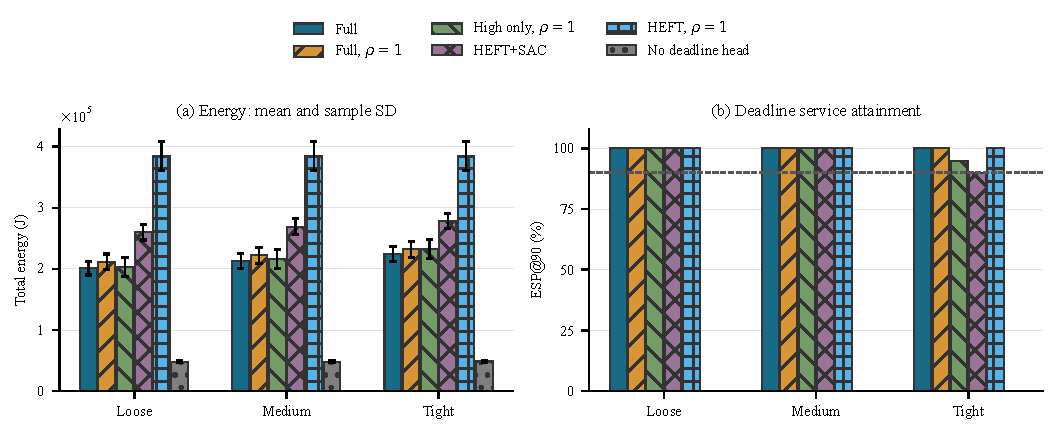
\includegraphics[width=\textwidth]{experiment_assets/ablation.pdf}
\caption{S26 structural ablations on 20 unseen test seeds.
Energy bars show the mean with sample-standard-deviation error bars;
the dashed line in the right panel marks the empirical ESP@90
service gate of 90\%. The very low energy of the no-deadline-head
variant is accompanied by zero ESP, so it is not a valid saving.
All results are conditional on one training run per trained variant.}
\label{fig:ablation}
\end{figure*}

\begin{table*}[t]
\centering
\caption{S26 ablations: energy (J), mean $\pm$ sample standard
deviation, and ESP@90 on 20 fixed test seeds. All reliability
attainment values are 100\%. Gray energy values fail the empirical
90\% ESP gate. Bold energy values are the lowest among feasible variants.}
\label{tab:ablation}
\scriptsize
\setlength{\tabcolsep}{4pt}
\renewcommand{\arraystretch}{1.12}
\begin{tabular}{@{}lrrrrrr@{}}
\toprule
& \multicolumn{2}{c}{Loose} & \multicolumn{2}{c}{Medium} & \multicolumn{2}{c}{Tight} \\
\cmidrule(lr){2-3}\cmidrule(lr){4-5}\cmidrule(l){6-7}
Variant & Energy (J) & ESP & Energy (J) & ESP & Energy (J) & ESP \\
\midrule
Full & \textbf{201,071.29 $\pm$ 11,024.15} & 100\% & \textbf{212,868.89 $\pm$ 12,545.21} & 100\% & \textbf{224,469.60 $\pm$ 12,838.52} & 100\% \\
Full, $\rho=1$ & 211,943.11 $\pm$ 12,478.92 & 100\% & 222,158.12 $\pm$ 13,499.18 & 100\% & 232,159.99 $\pm$ 13,122.15 & 100\% \\
High only, $\rho=1$ & 203,305.50 $\pm$ 15,853.78 & 100\% & 216,682.48 $\pm$ 15,727.77 & 100\% & 231,928.32 $\pm$ 15,565.62 & 95\% \\
HEFT+SAC & 260,141.52 $\pm$ 12,724.50 & 100\% & 269,414.45 $\pm$ 13,676.89 & 100\% & 278,090.85 $\pm$ 11,916.56 & 90\% \\
HEFT, $\rho=1$ & 384,508.56 $\pm$ 24,125.01 & 100\% & 384,508.56 $\pm$ 24,125.01 & 100\% & 384,508.56 $\pm$ 24,125.01 & 100\% \\
No deadline head & \textcolor{gray}{48,460.86 $\pm$ 1,806.66} & 0\% & \textcolor{gray}{48,458.77 $\pm$ 1,651.64} & 0\% & \textcolor{gray}{48,487.54 $\pm$ 1,662.90} & 0\% \\

\bottomrule
\end{tabular}
\end{table*}

\subsubsection{Contribution of Frequency Control}

Relative to evaluating Full at $\rho=1$, Full reduces mean energy
by 5.13\%, 4.18\%, and 3.31\% under Loose, Medium, and Tight
deadlines while retaining 100\% ESP. The benefit decreases as
deadlines become tighter, consistent with reduced room for slowing
execution. This intervention holds the learned network parameters
fixed, but not the complete placement trajectory: frequency changes
alter queues and can change later upper-level decisions. The measured
difference is therefore the net effect of frequency control under
the frozen policies, including its scheduling interactions.

\subsubsection{Contribution of Learned Placement}

Full consumes 22.71\%, 20.99\%, and 19.28\% less energy than
HEFT+SAC across the three regimes. Under Tight deadlines, HEFT+SAC
achieves 90\% ESP whereas Full achieves 100\%; both pass the stated
service gate, but with different robustness margins. HEFT+SAC itself
reduces energy by 27.68--32.34\% relative to HEFT at maximum frequency.
Thus, SAC can exploit slack under heuristic placement, but learned
placement is important to the lower energy of the complete system.
HEFT here is a reference heuristic, not a proved minimum-energy or
deadline-feasibility bound.

\subsubsection{Contribution of the Upper Deadline Estimator}

Removing the deadline head reduces mean energy to approximately
48,500 J but produces ESP $=0\%$ in all three regimes. The policy
therefore does not provide an admissible alternative to Full.
The full-frequency upper learner with its deadline head retained
achieves 100\%, 100\%, and 95\% ESP, providing a controlled contrast
with the no-head variant: both are independently trained at
full frequency. This comparison supports the necessity of
deadline-aware upper decisions in the tested system.
It does not individually identify the contribution of every queue,
critical-path, or credit-assignment term within that estimator.

Full also uses less energy than the independently trained upper-only
variant in every regime. Their Tight ESP values differ by one
successful test realization (20/20 versus 19/20). This observation
is consistent with a coordination benefit, but is not evidence of
training-seed-independent superiority of joint learning.

\subsection{Learning Dynamics}
\label{subsec:learning_dynamics}

Figure~\ref{fig:learning_dynamics} shows the recorded validation
energy and the minimum ESP across available validation blocks
during training. The curves use raw evaluation points without
smoothing and stop at the last saved evaluation; they are not
averages over repeated training runs. The Small configurations
reach high validation ESP earlier and fluctuate less afterward
than the Medium configurations. Low early energy coincides with
poor deadline attainment and should not be interpreted as a useful
energy optimum.

The Medium configurations continue to exhibit deadline fluctuations
after high-ESP checkpoints first appear. In particular, the last
M53 validation point is worse than some earlier points. Accordingly,
final testing uses a validation-selected checkpoint rather than the
last training episode. These curves demonstrate the importance of
constraint-aware checkpoint selection; they do not establish that
all four runs reached a stable optimization plateau.

\begin{figure*}[t]
\centering
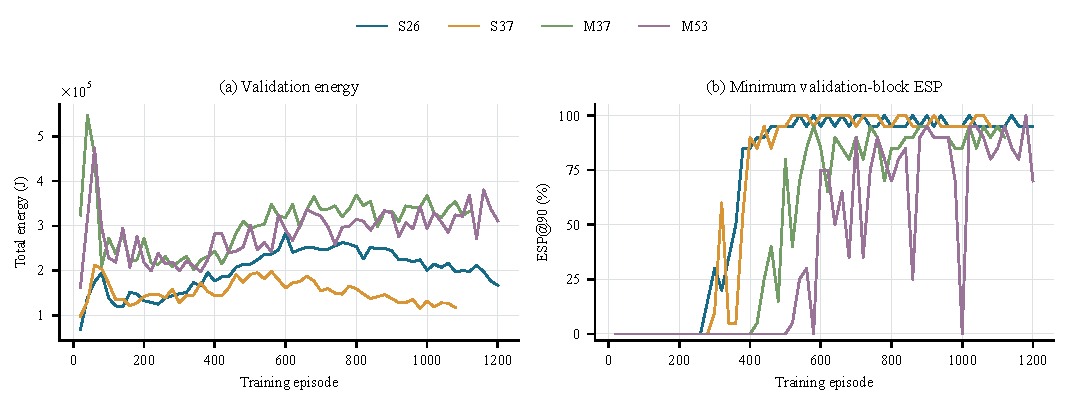
\includegraphics[width=\textwidth]{experiment_assets/learning_dynamics.pdf}
\caption{Recorded learning dynamics of the proposed method under
Medium deadlines. Energy is averaged over the available validation
blocks; deadline ESP is the minimum block value. Lines connect raw
evaluation points from one training run per configuration, without
smoothing or across-training-run confidence intervals. Curves stop
at the last saved evaluation, not necessarily the configured ceiling.}
\label{fig:learning_dynamics}
\end{figure*}

\subsection{Statistical Significance}
\label{subsec:significance}

We compare total energy using two-sided paired Wilcoxon signed-rank
tests. For each fixed test seed, relative energy reduction is
averaged equally over the four configurations and three deadline
regimes. This gives 20 seed-level contrasts, rather than treating
the 240 repeated condition-level observations as independent.
Table~\ref{tab:wilcoxon_energy} reports exact $p$-values and
corrections for the three baseline comparisons. All 20 aggregated
contrasts are positive for each baseline, which explains their
identical exact $p$-values. The comparisons remain significant
at level 0.05 after either correction.

These tests address energy differences across the evaluated
conditions, including conditions in which a baseline is infeasible.
They are not tests of deadline superiority or constrained optimality.
The inference is conditional on the selected policies and assumes
independent seed blocks and the signed-rank null's symmetry condition;
it does not quantify variability across independently trained policies.

\begin{table}[t]
\centering
\caption{Two-sided paired Wilcoxon signed-rank tests of total energy:
our method versus each baseline, using 20 seed-level contrasts.}
\label{tab:wilcoxon_energy}
\footnotesize
\setlength{\tabcolsep}{3.5pt}
\renewcommand{\arraystretch}{1.08}
\begin{tabular}{@{}lrrr@{}}
\toprule
Baseline & Raw $p$ & Bonferroni & BH--FDR \\
\midrule
DQN-Edge & $1.91\times10^{-6}$ & $5.72\times10^{-6}$ & $1.91\times10^{-6}$ \\
DReaM-DQN & $1.91\times10^{-6}$ & $5.72\times10^{-6}$ & $1.91\times10^{-6}$ \\
OOAC & $1.91\times10^{-6}$ & $5.72\times10^{-6}$ & $1.91\times10^{-6}$ \\
\bottomrule
\end{tabular}
\vspace{2pt}
\begin{minipage}{\columnwidth}
\footnotesize
Each contrast averages $(E_{\mathrm{baseline}}-E_{\mathrm{ours}})/
E_{\mathrm{baseline}}$ over 12 conditions for one seed. Both
corrections cover the three baseline comparisons. Energy significance
does not establish service-level feasibility.
\end{minipage}
\end{table}

\subsection{Scope and Limitations}
\label{subsec:experimental_limitations}

The four trained configurations demonstrate energy--service tradeoffs
on unseen workload realizations and different deadline distributions.
They do not demonstrate that one policy transfers unchanged across
all workflow sizes or server counts. Exploratory Medium-to-Large
transfer showed reduced deadline ESP, so uniform cross-scale
feasibility is not claimed. This limitation is distinct from the
within-configuration deadline-distribution tests in the main figure.

The current study also uses one training seed per reported trained
variant, historical differences in baseline checkpoint selection,
synthetically assigned workloads and data volumes, and a computation-only
energy objective. Reliability attainment is uniformly high under the
chosen fault rates, so these experiments do not establish a separate
energy or feasibility gain from reliability adaptation. Repeated
training, a fully uniform validation protocol, more demanding
reliability settings, and cross-scale deployment are needed before
making stronger reproducibility or generalization claims.
